\chapter{Motion-Aware Unitを用いた3波長を入力とした紫外線像の全球時系列予測}
  \section{実験概要}
    ここでは、171Å、193Åフィルターで得られたデータを追加で利用し、3波長の入力データから211Åの波長データに対する予測を行った。
    これらの波長は、太陽のコロナ領域における異なる温度帯を観測するためのものであり、予測モデルに多様な物理的情報を提供することが期待される。
    171Åの波長は、太陽のコロナにおける温度が約60万Kの領域を捉えるのに特化しており、193Åの波長は約100万Kの領域を捉える。
    これらの波長から得られる情報を組み合わせることにより、単一の波長では捉えられない層間の相互作用を捉え、より高い精度での予測を可能にすることを期待する。
    
    モデルには先の実験と同じく、MAUを用いる。入力は3波長、すなわち画像的には3チャンネルである。
    目的となる出力は211Åの波長のみであるが、MAUは3チャンネルを出力する。
    これは、「出力シークエンスのタイムステップ1以降では、直前のモデルの出力を入力データとして扱う」という動画予測モデルの一般的な性質によるものである。
    このような性質から、211Åの波長のみを出力として扱うために、出力された3チャンネルのうち、211Åの波長のみを抽出するという処理を行った
    図\ref{fig:exp2_concept}に本実験の概念図を示す。
    \begin{figure}[htbp]
      \centering
      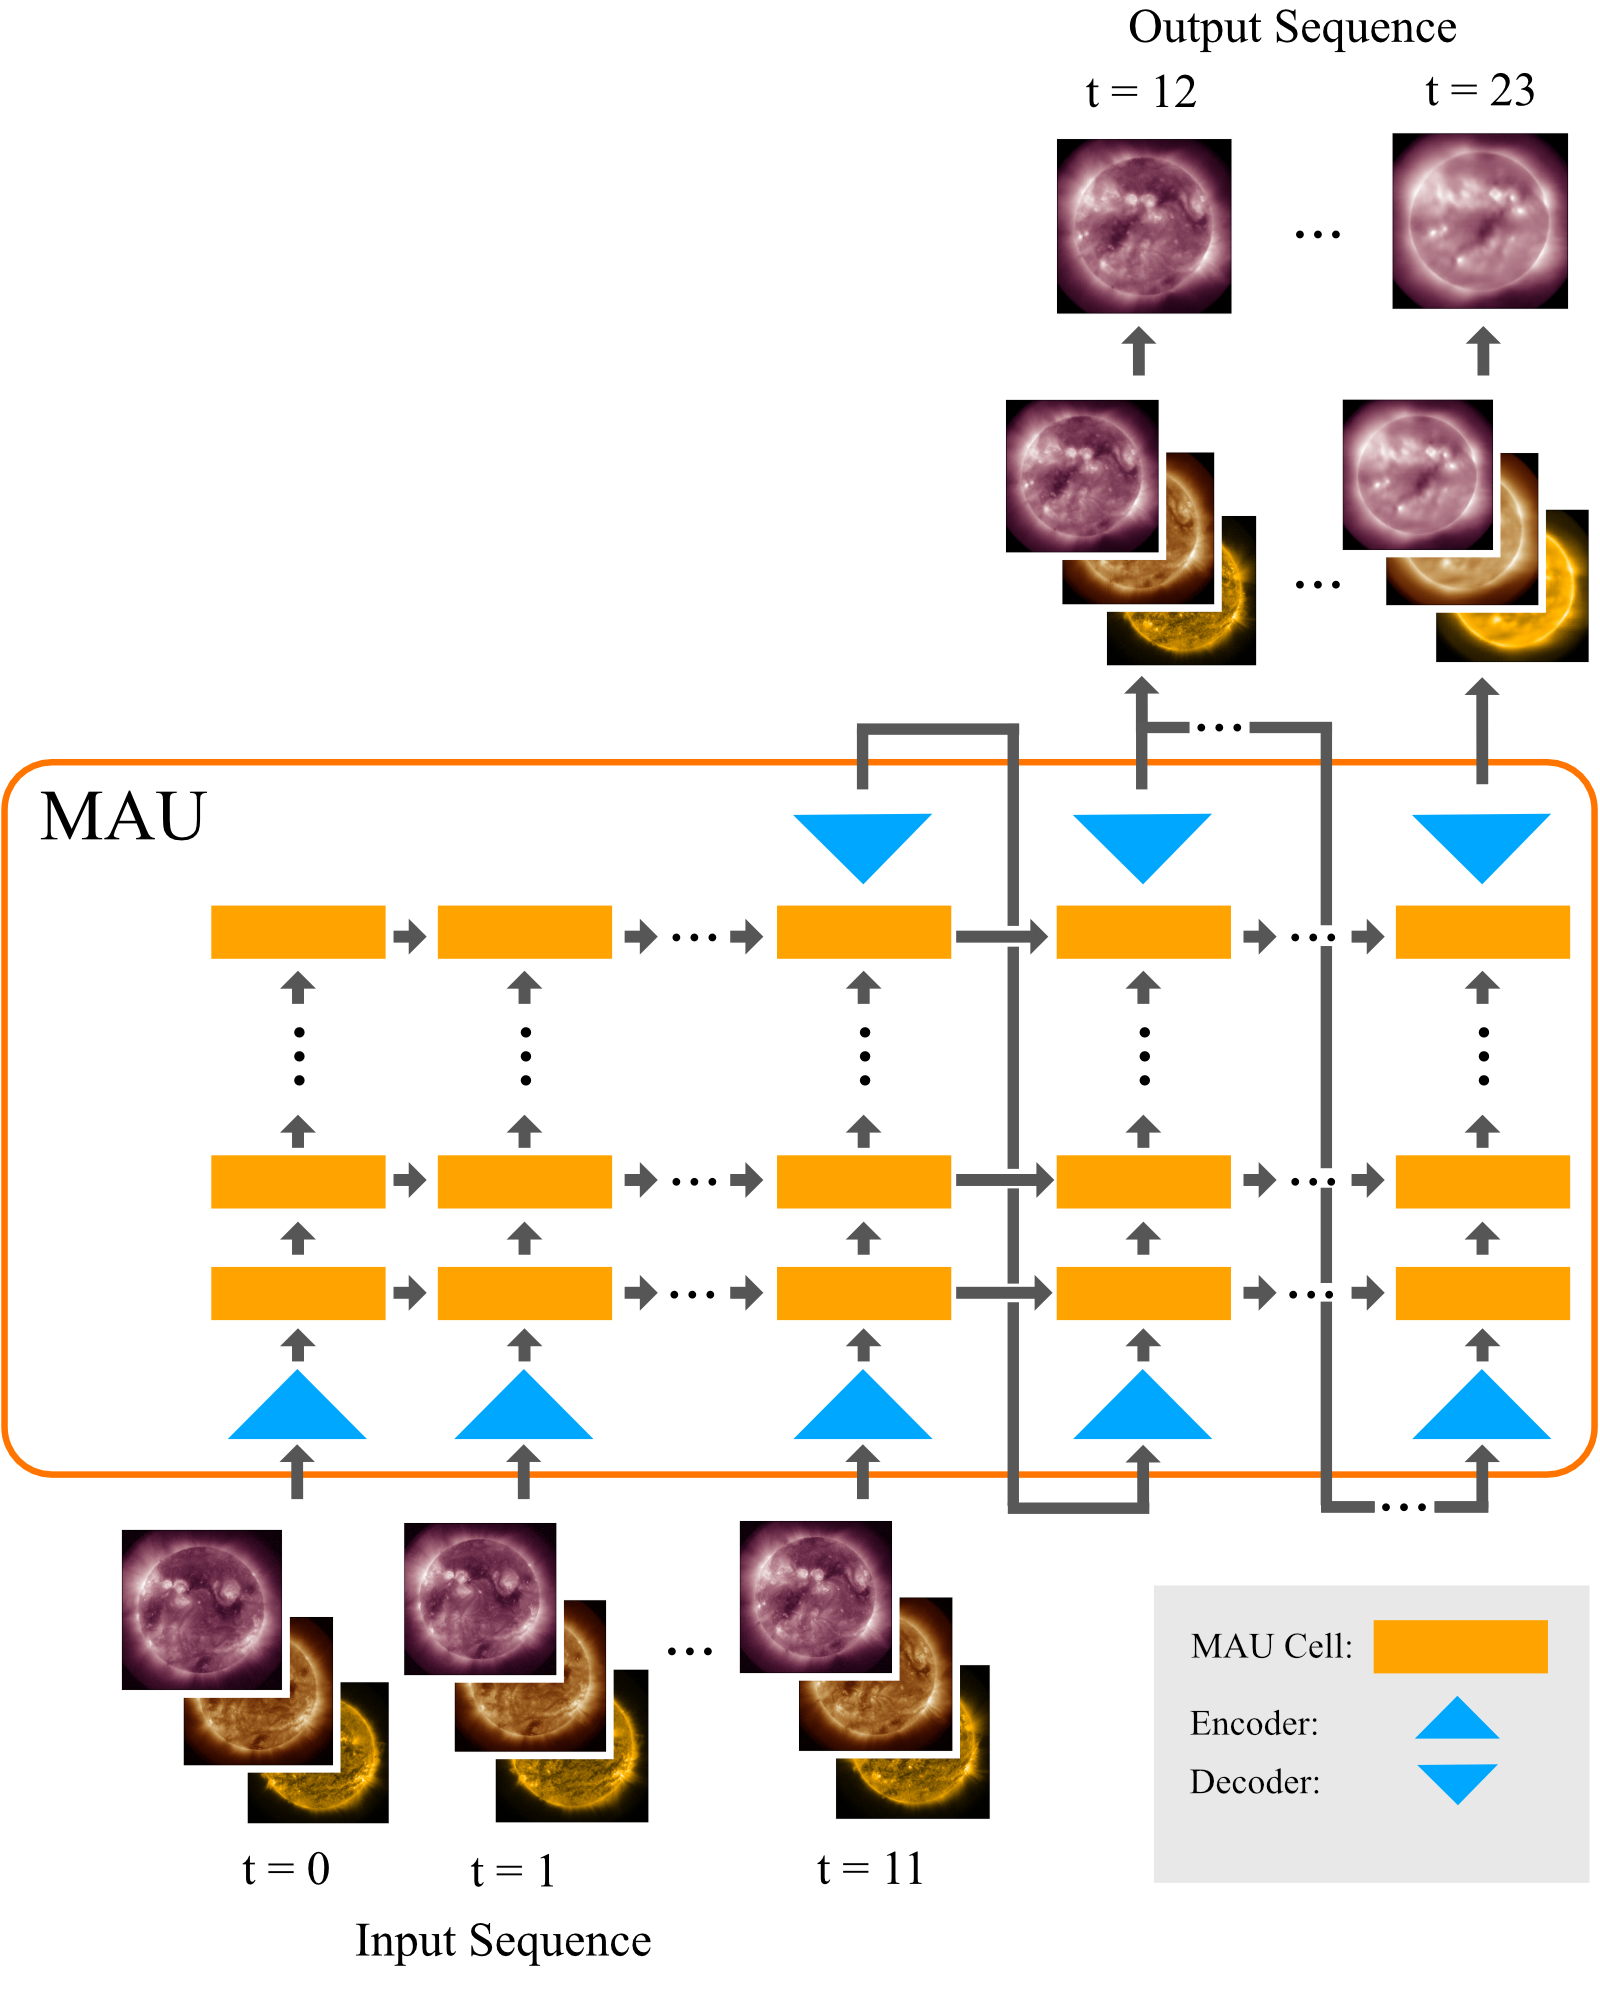
\includegraphics[width=\textwidth]{figures/exp2/exp2_concept.jpg}
      \caption{本実験の概念図。3波長の観測画像を入力として、211Åの波長の観測画像を予測する。}
      \label{fig:exp2_concept}
    \end{figure}

  \section{実験設定}
    各ハイパーパラメータの設定を表\ref{tab:exp2_hyperparameters}に示す。チャンネル数は入力波長に合わせて3である。
    バッチサイズは2に変更している。これは、NVIDIA RTX A6000のメモリ容量の制約によるものである。
    \begin{table}[htbp]
      \centering
      \begin{tabular}{lc}
      \hline
      ハイパーパラメータ & 値 \\
      \hline\hline
      バッチサイズ & 2 \\
      \hline
      エポック数 & 100 \\
      \hline
      学習率 & 0.0005 \\
      \hline
      損失関数 & MSE \\
      \hline
      チャンネル & 3 \\
      \hline
      カーネルサイズ & (5, 5) \\
      \hline
      MAU Cell数 & 16 \\
      \hline
      \end{tabular}
      \caption{本実験でのハイパーパラメータ設定。基本的には前実験と同様であるが、チャンネル数が1から3に変更されている。}
      \label{tab:exp2_hyperparameters}
    \end{table}
    データに関しても、データ数の増減による影響がないように、前回の実験と同じ期間のデータを用いた。欠損期間なども同様である。

  \section{学習の推移}
  学習は図\ref{fig:exp2_learn_progress}のように推移した。学習の初期段階では、学習データに対する損失関数の値が急激に減少しているが、学習が進むにつれて収束に向かって緩やかに減少していることがわかる。
  また、学習損失、検証損失ともに、安定的に減少していることがわかる。
  学習にはNVIDIA RTX A6000を用い、完了までに約60時間を要した。
  \begin{figure}[htbp]
    \centering
    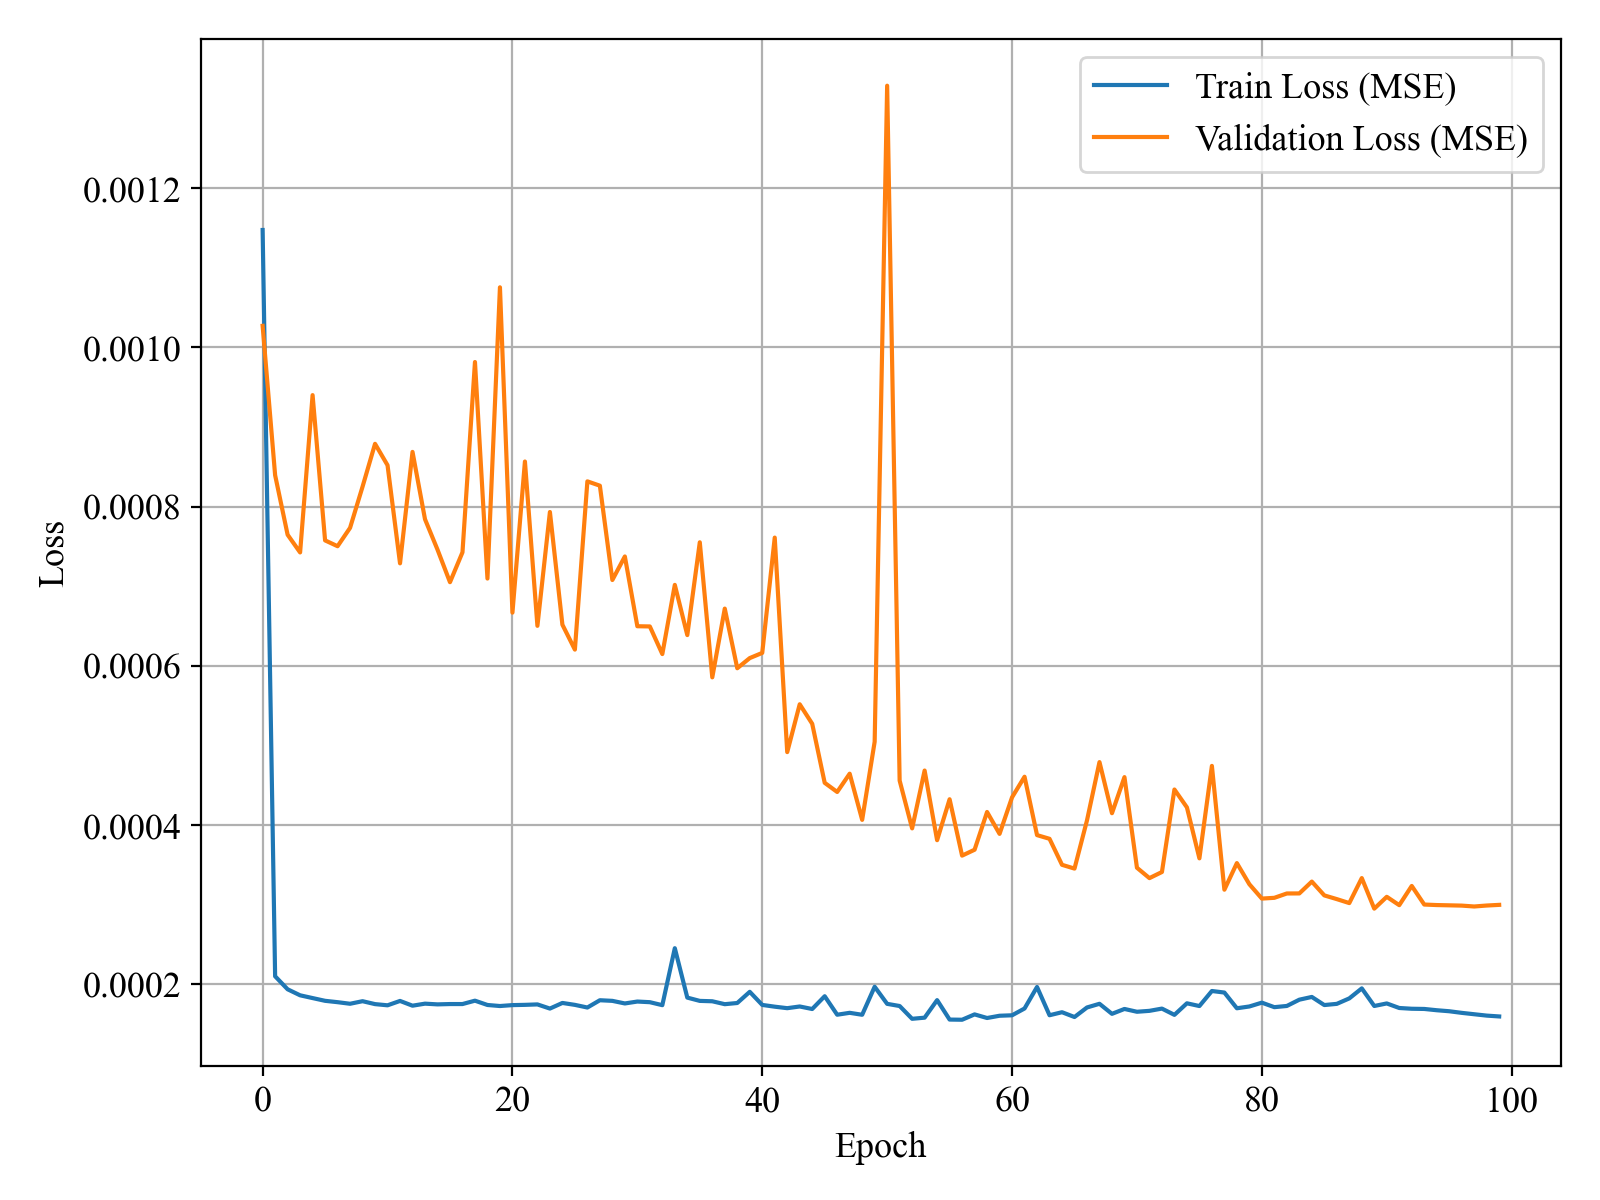
\includegraphics[width=0.8\textwidth]{figures/exp1/loss.png}
    \caption{本実験での、学習データ、検証データでの損失関数の推移。どちらも安定的に減少している。}
    \label{fig:exp2_learn_progress}
  \end{figure}

  \section{実験結果}
    図\ref{fig:exp2_gt}および図\ref{fig:exp2_pd}に、この実験での出力例を示す。

    \begin{figure}[htbp]
      \centering
      \vspace*{-2cm} % 上の余白を調整
      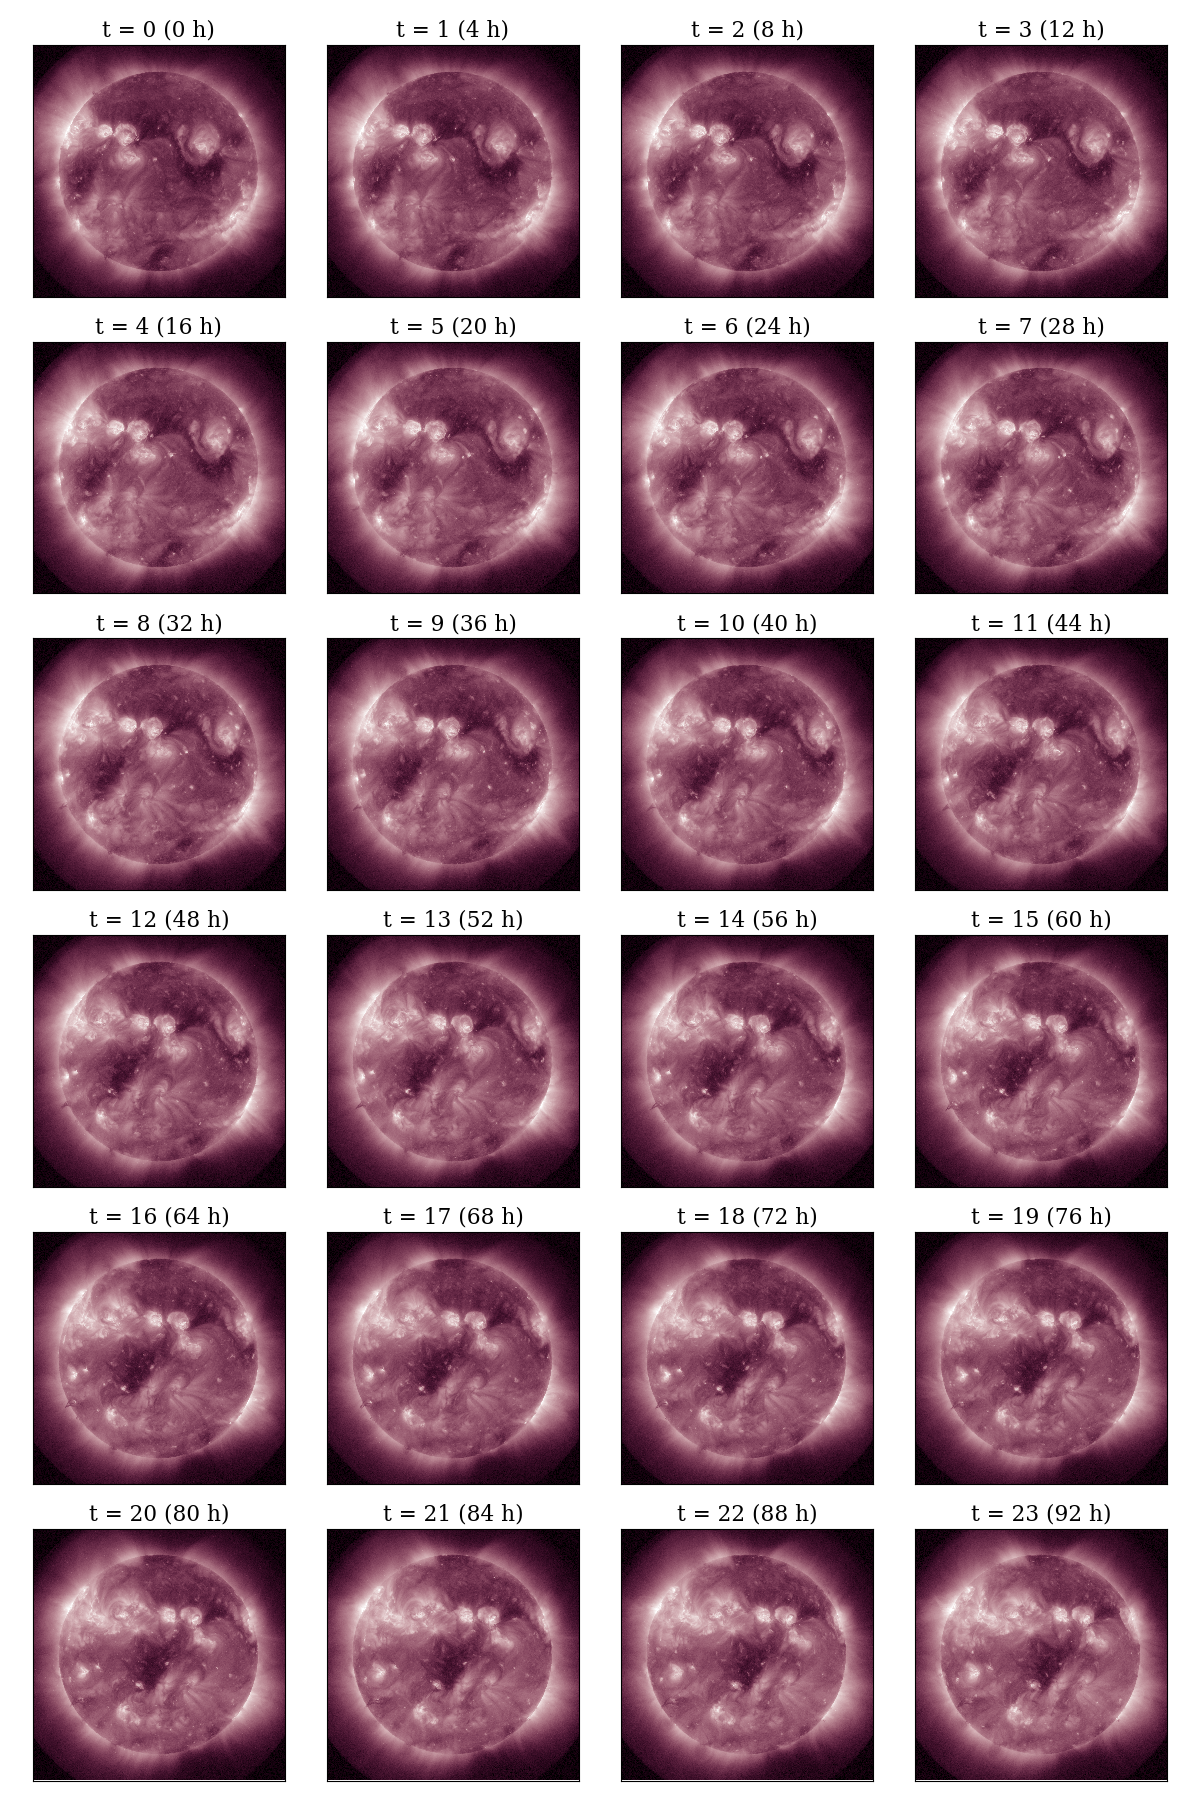
\includegraphics[width=0.95\textwidth]{figures/exp2/gt.png}
      \caption{実際の観測画像の例。2022年2月18日0時から2022年2月22日20時の期間から4時間毎にサンプリングされている。このt=0からt=11までをモデルに入力データとして渡している。モデルはその入力データを元に、t=12からt=23の12枚の画像を予測する。t=12以降の実際の観測画像はモデルに渡されない。}
      \vspace{-1cm} % 下の余白を調整
      \label{fig:exp2_gt}
    \end{figure}
    \begin{figure}[htbp]
      \centering
      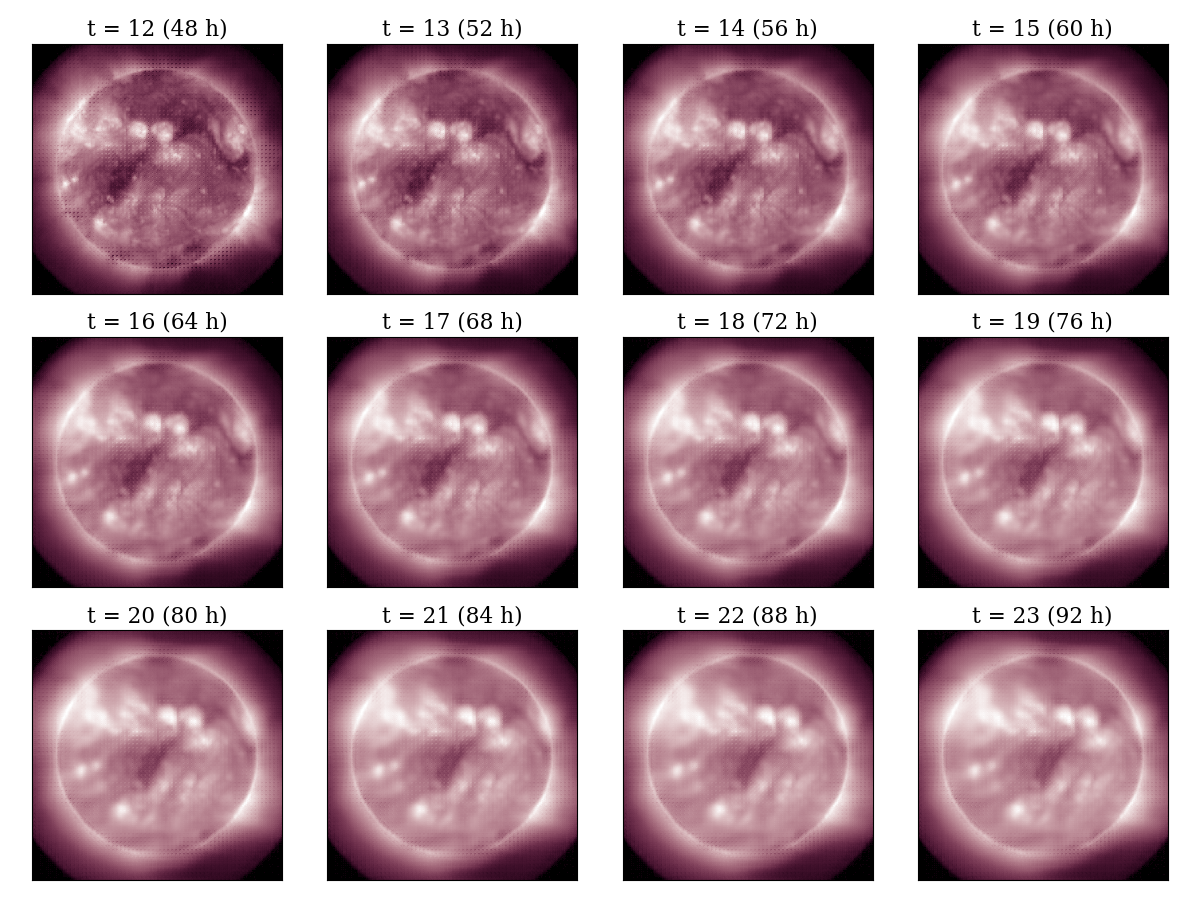
\includegraphics[width=0.95\textwidth]{figures/exp2/pd.png}
      \caption{MAUによる予測画像。対応するタイムステップtの観測画像(図\ref{fig:exp2_gt})と比較することでモデルの再現度を視覚的に評価することができる。大規模な構造は概ね実際の観測画像と合致している。モデルの特性により、時間経過とともに少しずつ予測が不安定になり、ぼやけた見た目になる。}
      \label{fig:exp2_pd}
    \end{figure}
    モデルの出力は、視覚的には実際の観測画像と概ね合致している。
    この実験における評価では、前回の実験と同様の評価を行った。
  
% *************************************************************************************************************
    \subsection{全球での評価}
      はじめに全球での評価を行った。
      前回実験と同様に、まず輝度強度の平均値と実際の平均値との誤差、SSIMを計算した。さらに単純差動回転モデルとの比較も行った。
      また、これらの値の時間経過に対する変化を観察し、より不確定性の高い将来の予測に対しても動画予測モデルが有効であるかを検証した。

      \subsubsection{平均輝度の再現}
        モデルの出力の全球での平均輝度と、実際の観測画像との絶対誤差の推移を図\ref{fig:exp2_error}に示す。
        これは、50のテストセットに対して、各テストセットに含まれる各画像の全球での平均輝度を計算し、その時間ステップごとの平均値を取ったものである。
        また、前回実験と同様に、モデルの予測性能をさらに詳細に評価するために、シンプルな差動回転モデルとの比較を行った。
        \begin{figure}[htbp]
          \centering
          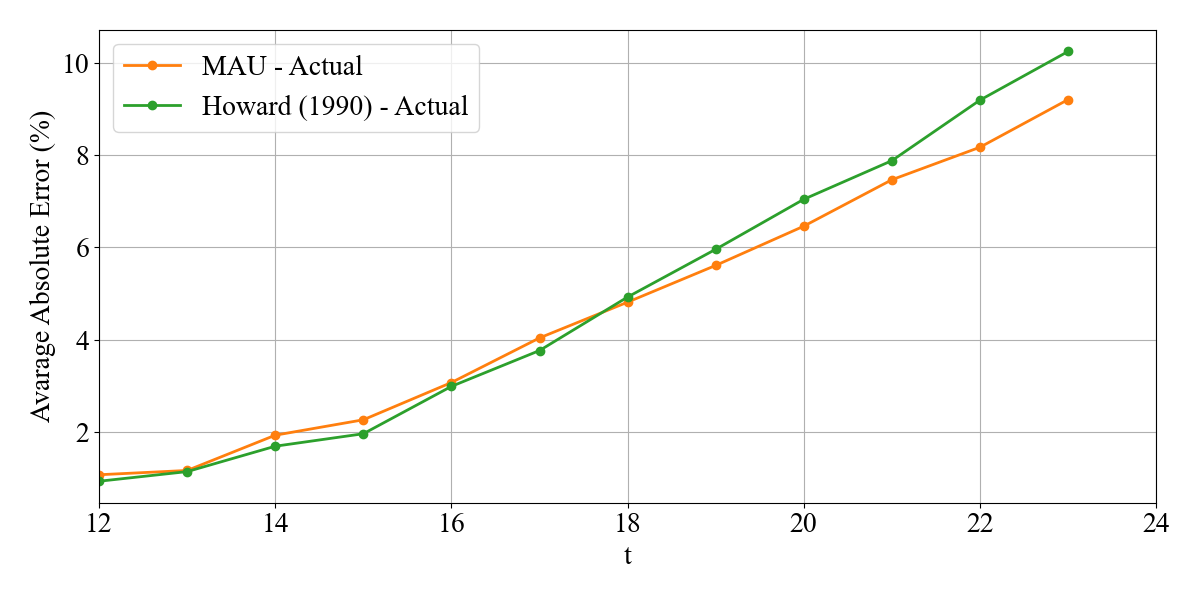
\includegraphics[width=\textwidth]{figures/exp2/error_dr.png}
          \caption{MAUによるテストセットの予測画像と実際の観測画像の平均絶対誤差(オレンジ)と、単純差動回転モデルと実際の観測画像の平均絶対誤差(緑)。}
          \label{fig:exp2_error}
        \end{figure}
        
        さらに、出力シークエンスの最後のタイムステップにおいて、単純差動回転モデルによるシミュレーションと、実際の観測画像との差異を観察し、動画予測モデルによる出力と比較した。
        このタイムステップは、出力の最後のタイムステップであり、最も不確定性の高い予測である。
        その散布図\ref{fig:exp2_dr_scatter}に示す。
        \begin{figure}[htbp]
          \begin{subfigure}[b]{0.55\textwidth}
            \centering
            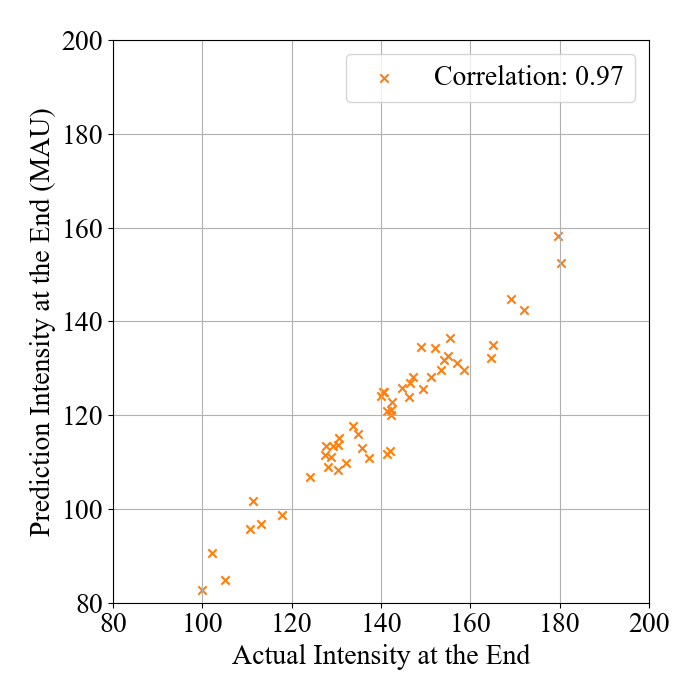
\includegraphics[width=\textwidth]{figures/exp2/intensity_scatter_gt_pd.png}
            \caption{MAUによる、テストセットの最終ステップにおける全球平均輝度の予測対実測の散布図。計算された相関係数は0.97である。}
          \end{subfigure}
          \begin{subfigure}[b]{0.55\textwidth}
            \centering
            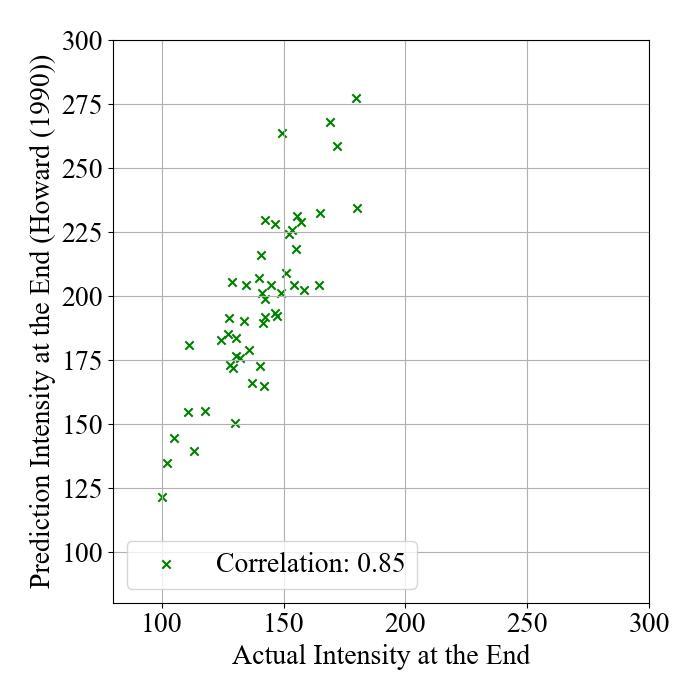
\includegraphics[width=\textwidth]{figures/exp2/intensity_scatter_gt_dr.png}
            \caption{単純差動回転モデルによる、テストセットの最終ステップにおける全球平均輝度の予測対実測の散布図。計算された相関係数は0.85である。}
          \end{subfigure}
          \label{fig:exp2_dr_scatter}
          \caption{予測対実測の散布図。縦軸が予測から計算された平均輝度強度、横軸が実際の観測画像から計算された平均輝度強度を表す。}
        \end{figure}

      \subsubsection{画像類似度}
        前回実験と同様に、画像内での構造的再現度とその時間的変化を評価するために、モデルの出力と対応する時間ステップの実際の観測画像の間のSSIMを計算した。
        SSIMの推移を図\ref{fig:exp2_ssim}に示す。画像類似度は、全球での平均輝度と同様に、全球に対してのみ行い、画像中の背景や外縁部からはみ出すコロナなどはその計算に含まれない。
        \begin{figure}[htbp]
          \centering
          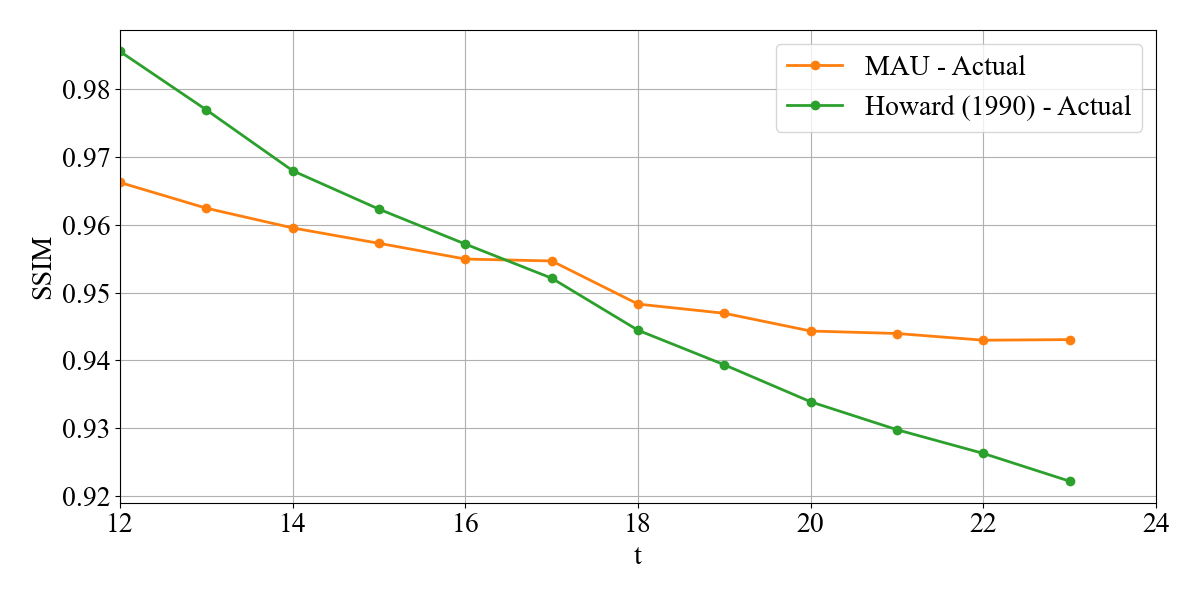
\includegraphics[width=\textwidth]{figures/exp2/average_ssim.png}
          \caption{テストセットでのSSIMの時間推移。SSIMは0から1の値を取り、二つの画像が類似するほど1に近づく。横軸が時間ステップ、縦軸がSSIMを表す。}
          \label{fig:exp2_ssim}
        \end{figure}

% *************************************************************************************************************
        
      \subsection{経度依存性の評価}
        前回実験と同じく、予測性能が経度ごとにばらつきがあるかを確認するために、経度ごと予測の再現度を評価した。分割の方法は前回実験と同様である。
        評価指標には、平均輝度の誤差と、その単純差動回転モデルとの比較を用いた。

        \subsubsection{平均輝度の再現}
          ここでは、全てのテストセットで各セクターごとの平均輝度を計算し、対応する時間ステップの実際の観測画像との絶対誤差を計算した。
            誤差率の時間推移を図\ref{fig:lng_error}に示す。同時に単純差動回転モデルの経度ごとの画像類似度も計算した。
            \begin{figure}[htbp]
              \begin{subfigure}{0.5\textwidth}
                \centering
                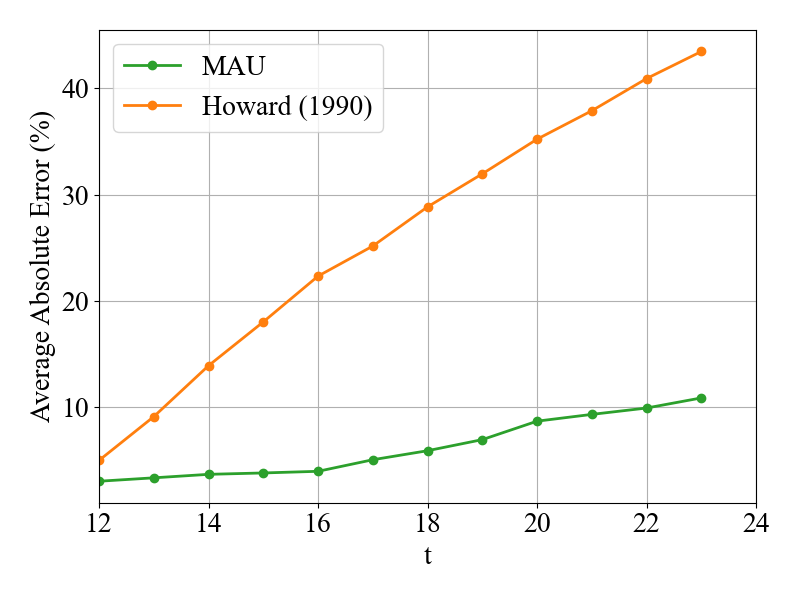
\includegraphics[width=\textwidth]{figures/exp2/lng_error_1.png}
                \caption{-90度から-54度}
              \end{subfigure}%
              \begin{subfigure}{0.5\textwidth}
                \centering
                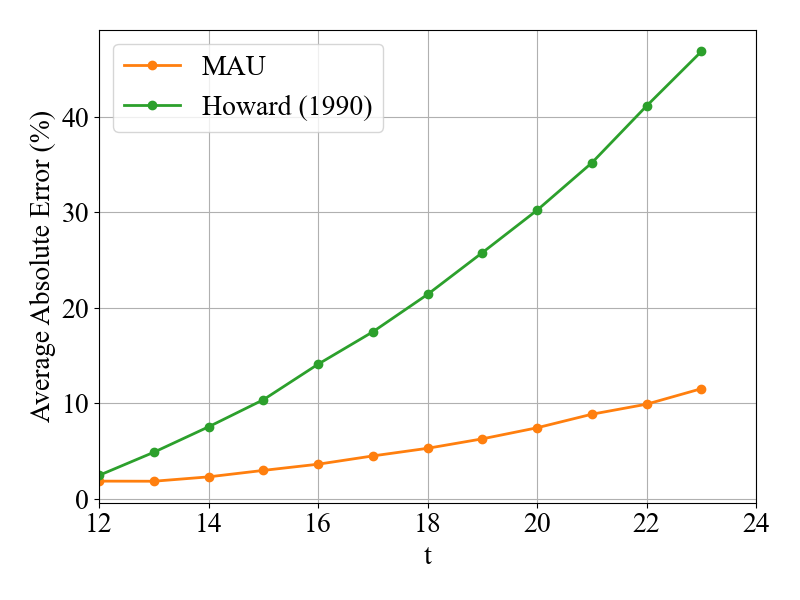
\includegraphics[width=\textwidth]{figures/exp2/lng_error_2.png}
                \caption{-54度から-18度}
              \end{subfigure} \par
              \begin{subfigure}{0.5\textwidth}
                \centering
                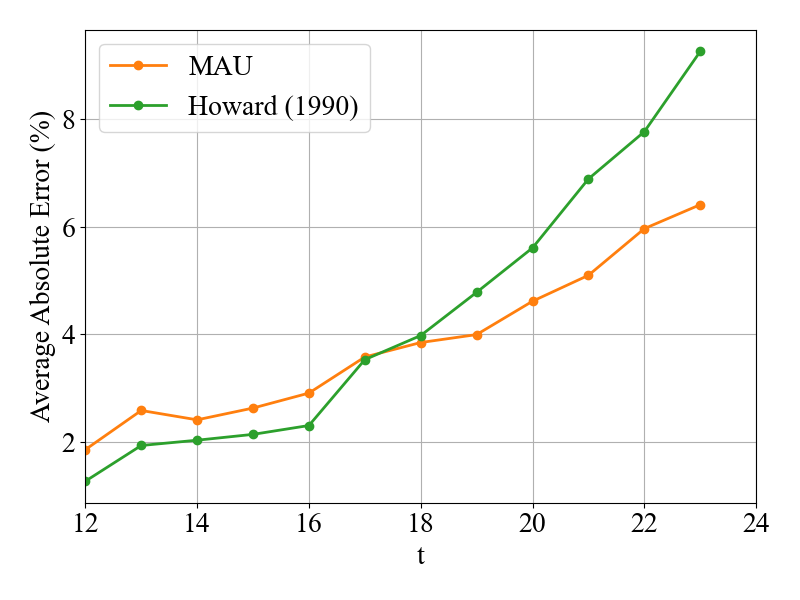
\includegraphics[width=\textwidth]{figures/exp2/lng_error_3.png}
                \caption{-18度から18度}
              \end{subfigure}%
              \begin{subfigure}{0.5\textwidth}
                \centering
                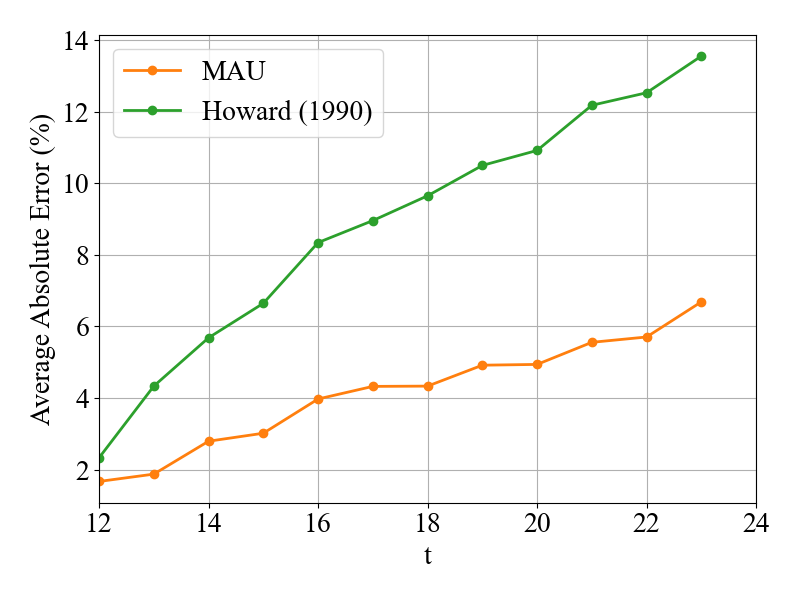
\includegraphics[width=\textwidth]{figures/exp2/lng_error_4.png}
                \caption{18度から54度}
              \end{subfigure} \par
              \begin{subfigure}{0.5\textwidth}
                \centering
                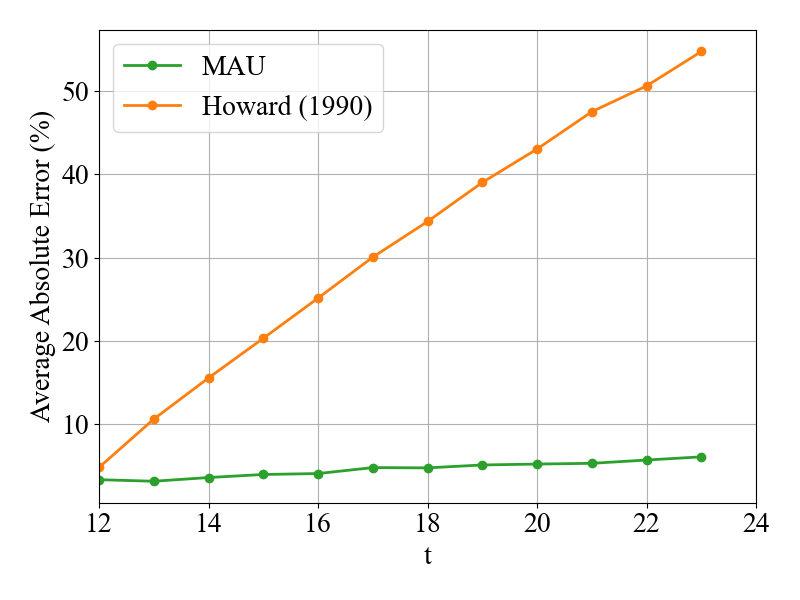
\includegraphics[width=\textwidth]{figures/exp2/lng_error_5.png}
                \caption{54度から90度}
              \end{subfigure}
              \caption{分割された各セクターにおける平均輝度の絶対誤差の時間推移。横軸が時間ステップ、縦軸が平均絶対誤差を表す。各グラフで縦軸の範囲が異なる。緑線がMAUによる予測から計算された絶対誤差、オレンジ線が単純差動回転モデルによるシミュレーションから計算された絶対誤差を表す。}
              \label{fig:lng_error}
            \end{figure}
          
        \subsubsection{画像類似度}
          全球での場合と同様に、経度ごとにも画像類似度を計算した。その時間推移を図\ref{fig:lng_ssim}に示す。
          同時に単純差動回転モデルの経度ごとの画像類似度も計算した。
          \begin{figure}[htbp]
            \begin{subfigure}{0.5\textwidth}
              \centering
              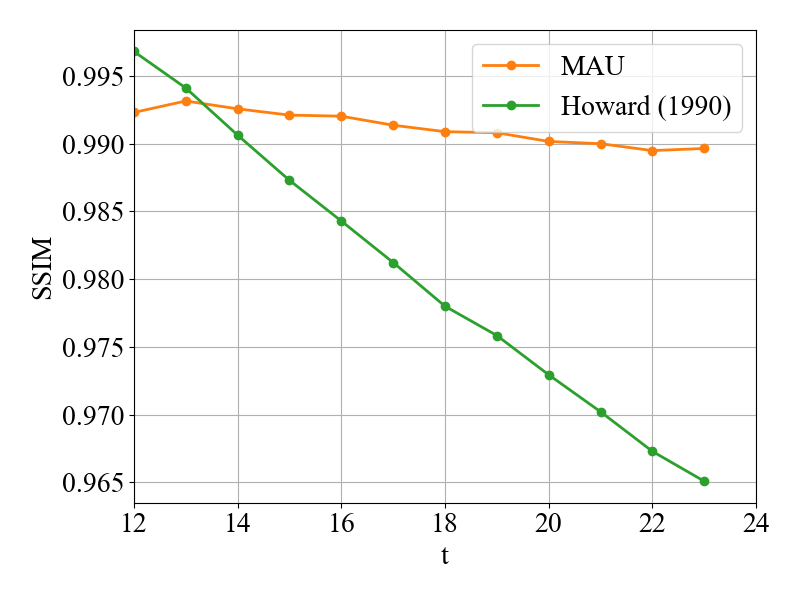
\includegraphics[width=\textwidth]{figures/exp2/lng_ssim_1.png}
              \caption{-90度から-54度}
            \end{subfigure}
            \begin{subfigure}{0.5\textwidth}
              \centering
              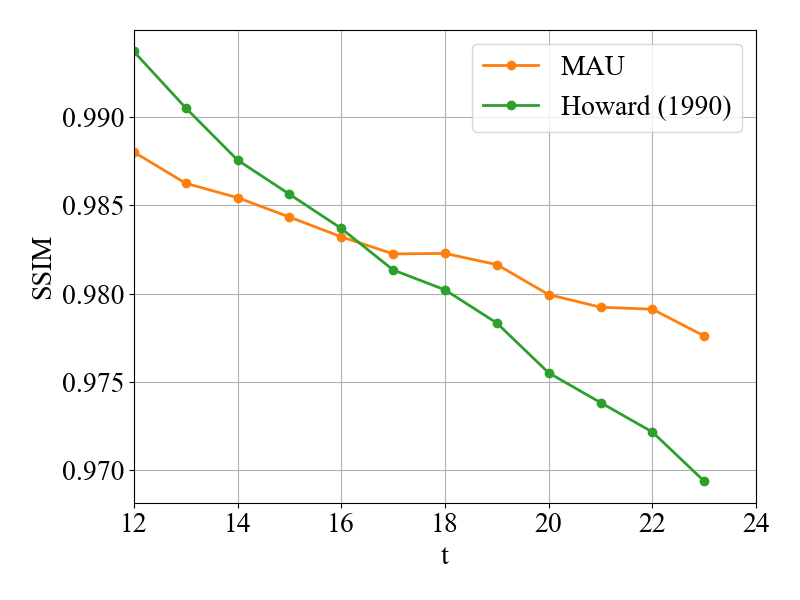
\includegraphics[width=\textwidth]{figures/exp2/lng_ssim_2.png}
              \caption{-54度から-18度}
            \end{subfigure} \par
            \begin{subfigure}{0.5\textwidth}
              \centering
              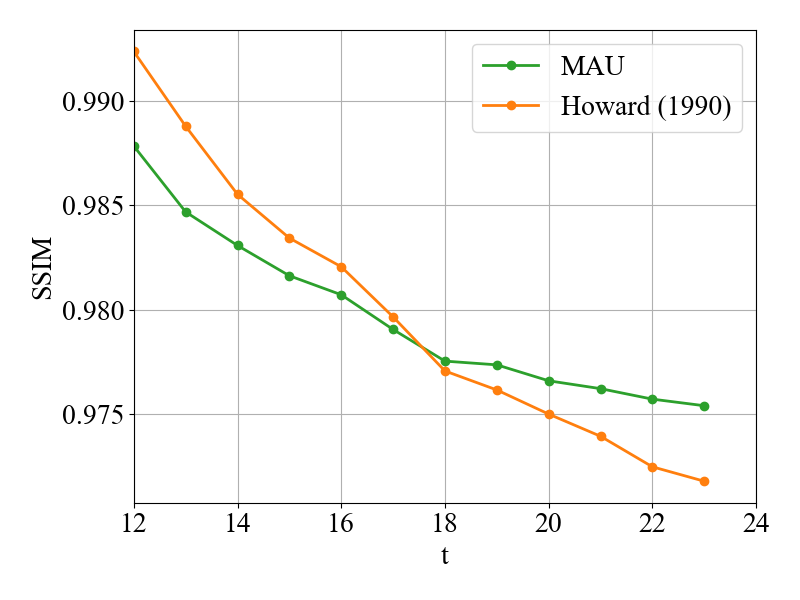
\includegraphics[width=\textwidth]{figures/exp2/lng_ssim_3.png}
              \caption{-18度から18度}
            \end{subfigure}
            \begin{subfigure}{0.5\textwidth}
              \centering
              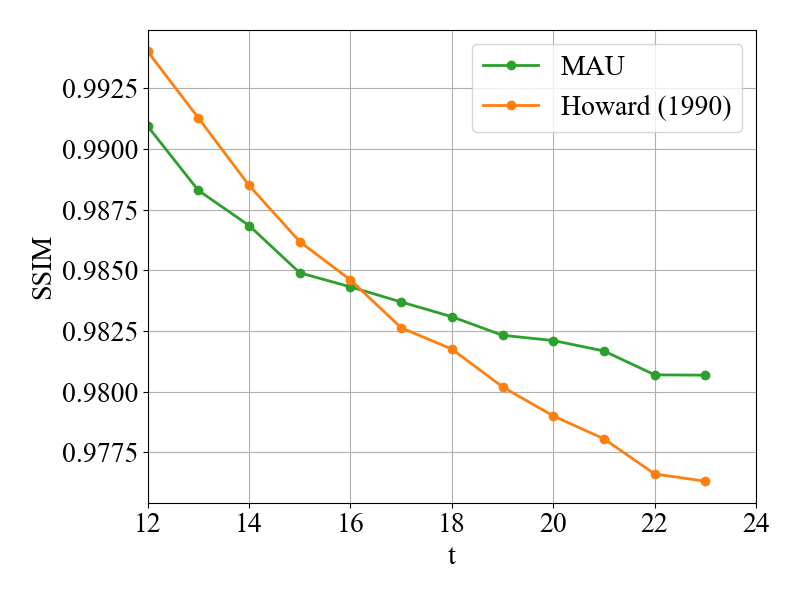
\includegraphics[width=\textwidth]{figures/exp2/lng_ssim_4.png}
              \caption{18度から54度}
            \end{subfigure} \par
            \begin{subfigure}{0.5\textwidth}
              \centering
              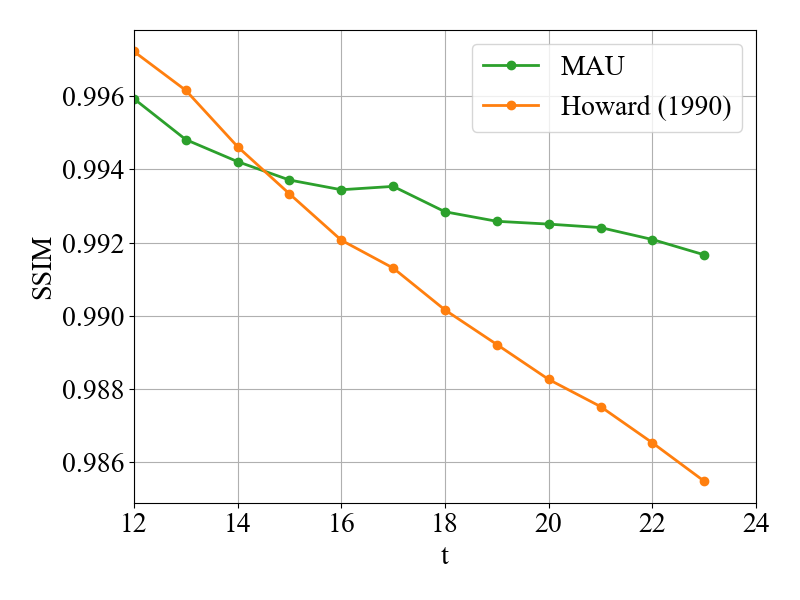
\includegraphics[width=\textwidth]{figures/exp2/lng_ssim_5.png}
              \caption{54度から90度}
            \end{subfigure}
          \label{fig:exp2_ssim}
          \caption{分割された各セクターにおけるSSIMの時間推移。横軸が時間ステップ、縦軸がSSIMを表す。各グラフで縦軸の範囲が異なる。緑線がMAUによる予測から計算されたSSIM、オレンジ線が単純差動回転モデルによるシミュレーションから計算されたSSIMを表す。}
        \end{figure}

% *************************************************************************************************************

    \subsection{東側外縁部に対する評価}
      \subsubsection{視覚的評価}
        ここでは、動画予測モデルが、東側外縁部から出現する活動領域に対して、どのような予測を行っているかを視覚的に評価する。
        いくつかの例を図\ref{fig:exp1_limb_example_1}および\ref{fig:exp2_limb_example_2}に示す。ここで示す画像は、左列が入力シークエンスの最終データ、中央列がその24時間後の予測画像、右列がその48時間後の予測画像である。
        \begin{figure}[htbp]
          \centering
          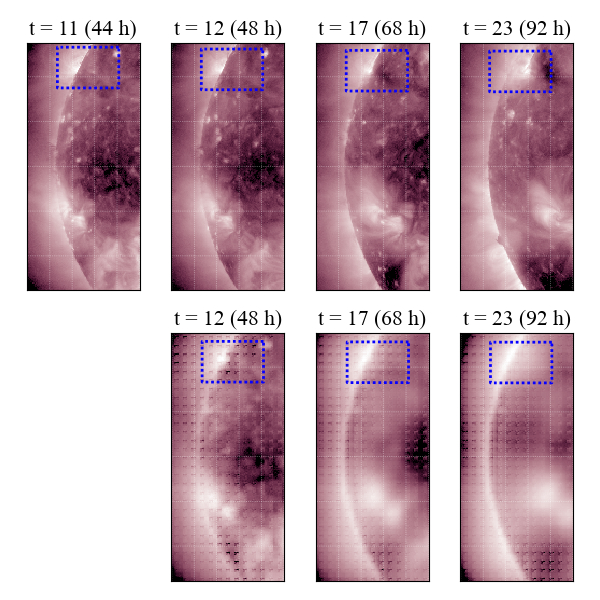
\includegraphics[width=\textwidth]{figures/exp2/limb_sample_3_caption.jpg}
          \caption{東側外縁部から出現する活動領域に対する予測の例。左列が入力シークエンスの最終データ、中央列がその24時間後の予測画像、右列がその48時間後の予測画像である。}
          \label{fig:exp1_limb_example_1}
        \end{figure}
        \begin{figure}[htbp]
          \centering
          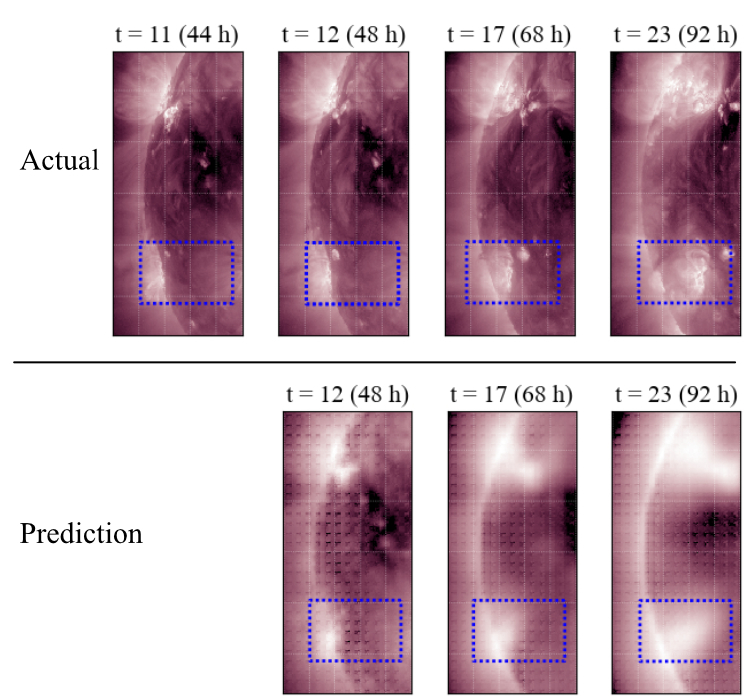
\includegraphics[width=\textwidth]{figures/exp2/limb_sample_12_caption.jpg}
          \caption{東側外縁部から出現する活動領域に対する予測の例。左列が入力シークエンスの最終データ、中央列がその24時間後の予測画像、右列がその48時間後の予測画像である。}
          \label{fig:exp2_limb_example_2}
        \end{figure}

      \subsubsection{散布図}
        さらに、東側外縁部に対する評価を行うために、予測対実測の散布図を作成した。その結果を図\ref{fig:exp2_limb_scatter}に示す。
        左は、MAUによる予測画像の東側外縁部の平均輝度と、実際の観測画像の東側外縁部の平均輝度の散布図である。

        \begin{figure}[htbp]
          \begin{subfigure}[b]{0.55\textwidth}
            \centering
            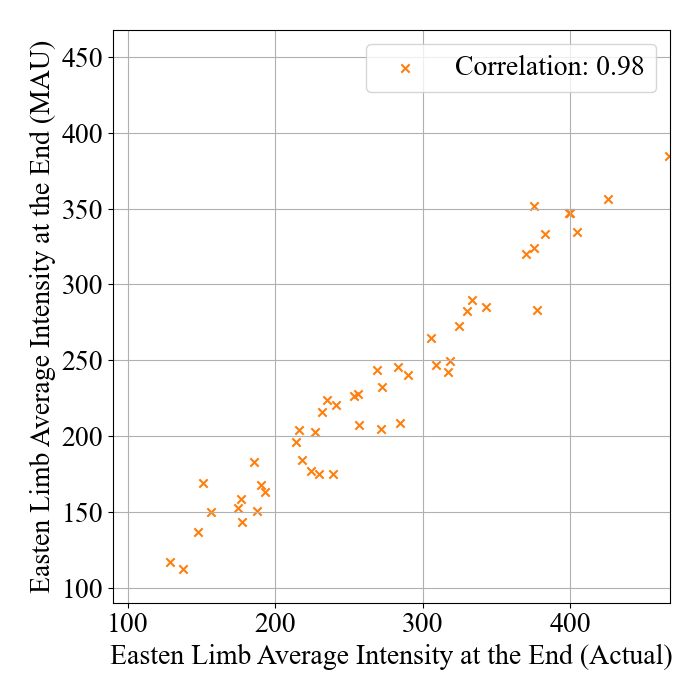
\includegraphics[width=\textwidth]{figures/exp2/limb_scatter_gt_pd.png}
            \caption{すべてのテストセットの、最終タイムステップでの東側外縁部の平均輝度の予測対実測の散布図。横軸が実際の観測画像から計算された平均輝度強度、縦軸がMAUによる予測から計算された平均輝度強度を表す。計算された相関係数は0.98である。}
          \end{subfigure}
          \begin{subfigure}[b]{0.55\textwidth}
            \centering
            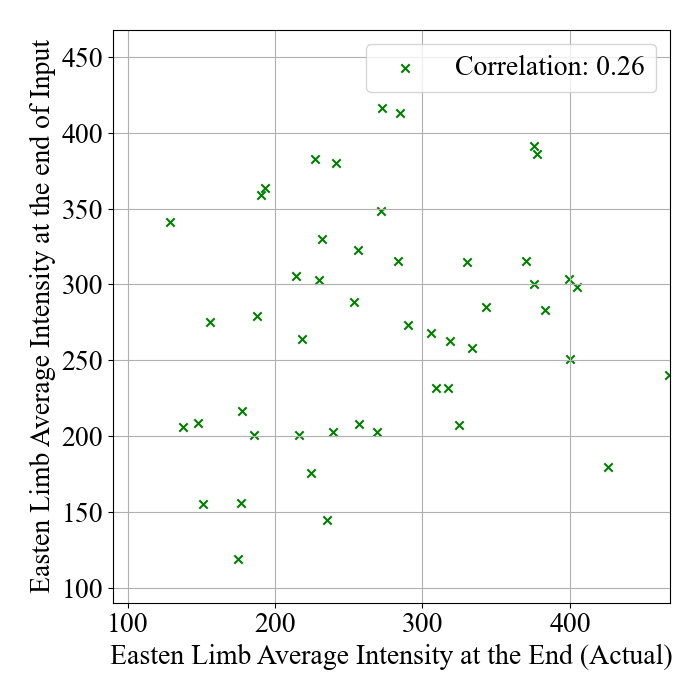
\includegraphics[width=\textwidth]{figures/exp2/limb_scatter_gt_sp.png}
            \caption{すべてのテストセットでの、最終タイムステップでの東側外縁部の平均輝度の実測値と、その48時間前の実測値の散布図。横軸が実際の観測画像から計算された平均輝度強度、縦軸がMAUによる予測から計算された平均輝度強度を表す。計算された相関係数は0.26である。}
          \end{subfigure}
          \label{fig:exp2_limb_scatter}
        \end{figure}
        
    \subsection{まとめ}
      \begin{table}[htbp]
        \centering
        \caption{本実験での各評価の結果。MAUは、本研究で使用した動画予測モデルによる予測に対する評価、Howard (1990)は、単純差動回転モデルによるシミュレーションに対する評価を表す。}
        \begin{tabular}{lcccccc}
        \hline
        評価指標 & 全球 & \multicolumn{5}{c}{経度ごと} \\
        \cline{3-7}
         &  & -90 to -54 & -54 to -18 & -18 to 18 & 18 to 54 & 54 to 90 \\
        \hline\hline
        平均輝度絶対誤差↓ & & & & & & \\
        \quad MAU - 1波長 & 0.05 & 0.04 & 0.03 & 0.05 & 0.06 & 0.04 \\
        \quad MAU - 3波長 & 0.9 & 0.88 & 0.89 & 0.87 & 0.85 & 0.86 \\
        \quad Howard (1990) & 0.06 & 0.05 & 0.04 & 0.06 & 0.07 & 0.05 \\
        \hline
        SSIM↑ & & & & & & \\
        \quad MAU - 1波長 & 0.9 & 0.88 & 0.89 & 0.87 & 0.85 & 0.86 \\
        \quad MAU - 3波長 & 0.9 & 0.88 & 0.89 & 0.87 & 0.85 & 0.86 \\
        \quad Howard (1990) & 0.85 & 0.87 & 0.86 & 0.84 & 0.83 & 0.85 \\
        \hline
        \end{tabular}
        \label{tab:exp2_result}
      \end{table}


  \section{考察}
